\documentclass[twocolumn]{aastex62}
\newcommand{\vdag}{(v)^\dagger}
\newcommand\aastex{AAS\TeX}
\newcommand\latex{La\TeX}
\usepackage{amsmath}
\usepackage{physics}
\usepackage{hyperref}
\usepackage{natbib}
\usepackage[T1]{fontenc}
\usepackage[english]{babel}
\usepackage[utf8]{inputenc}

\begin{document}

\title{Solving Eigenvalue Problems by Means of the Jacobi Algorithm}

\author{Håkon Tansem}

\author{Nils-Ole Stutzer}

\author{Bernhard Nornes Lotsberg}

\begin{abstract}
\end{abstract}

\section{Introduction} \label{sec:intro}
When solving problems in science and mathematics an ever recurring problem is to
solve integrals. Integrals are found in all sorts of manners, e.g. when
computing expectation values in quantum mechanics. In this paper we will
consider ways of solving an example of a six dimensional expectation value
problem from quantum mechanics integral in several different ways. We will
consider a brute force Gauss-Legendre quadrature, an improved Gauss-Laguerre
quadrature, a brute force monte carlo integration and a monte carlo integration
with importance sampling as shown by \cite{press:2007} and \cite{jensen:2015}.
The resulting integrals will be compared to the analytical solution and the run
times are compared, in order to find which method is most efficient.

In the theory section we present needed theory wich we discuss how to implement
in the method section. The results are presented in the results section and
discussed in the discussion section.

\section{Theory} \label{sec:theory}
\subsection{The integral}\label{subsec:integral}
Before stating the needed integration methods we used we present the integral to
integrate. Assuming the wave function of two electrons can be modelled as a
single-particle wave function in a hydrogen atom, the wave function of the $i$th
electon in the 1 $s$ state is given by 
\begin{align}
	\psi_{1,s}(\vec{r}_i) = e^{-\alpha r_i},
\end{align}
where the dimensionless position
\begin{align}
	\vec{r}_i = x_i \hat{e}_x + y_i\hat{e}_y + z_i\hat{e}_z
\end{align} 
with orthogonal unit vectors $\hat{e}_i$.

The distance $r_i = \sqrt{x_i^2 + y_i^2 + z_i^2}$ and we let the parameter
$\alpha = 2$ corresponding to the charge of a helium $Z = 2$. Then the ansats
for the wave function for two electrons is given by the product of the two 1 $s$
wave functions 
\begin{align}
	\Psi(\vec{r}_1, \vec{r}_2) = e^{-\alpha(r_1 + r_2)}.
\end{align}
We now want to find the expectation value of the correlation energy between
electrons which repel each other by means of the Coulomb interaction as 
\begin{align}
\langle \frac{
1}{\vec{r}_1 - \vec{r}_2}\rangle = \int d\vec{r}_1d\vec{r}_2 e^{-2\alpha(r_1 + r_2)}\frac{1}{|\vec{r}_1 - \vec{r}_2|}.
\label{eq:integral}
\end{align}
This integral has an analytical solution $5\pi^2/16^2$, which we can later
compare numerical results to.
\subsection{Brute Force Gauss-Legendre Quadrature}\label{subsec:brute_force_gauss}
The following theory and derivations of the integration methods presented
follows closely \citep[Ch. 5.3]{jensen:2015}. 

The essence of Gaussian Quadrature (GQ) is to approximate an integral 
\begin{align}
	I = \int f(x) dx \approx \sum^N_{i = 1} \omega_i f(x_i),
	\label{eq:quadrature}
\end{align} 
for some weights $\omega_i$ and grid points $x_i$. The grid points and wights
are obtained through the zeros of othogonal polynomials. These polynomials are
orthogonal on some intervale, for instance $[-1, 1]$ for Legendre polynomials.
Since we must find $N$ grid points and weigths, we must fit $2N$ parameters.
Therefore we must approximate the integrand $f(x)$ by a polynomial of degree
$2N-1$, i.e. $f(x) \approx P_{2N-1}(x)$. Then the integral 
\begin{align}
	I \approx \int P_{2N-1}(x)dx = \sum^{N-1}_{i=0}P_{2N-1}(x_i) \omega_i.
\end{align} 
GQ can integrate all polynomials of degree up to $2N-1$ exactelly, we thus get
an equallity when approximating the integral of $P_{2N-1}$. 

If we choose to expande the polynomial $P_{2N-1}$ in terms of the Legendre
polynomials $L_N$, we can through polynomial devision write 
\begin{align}
	P_{2N-1} = L_N(x)P_{N-1}(x) + Q_{N-1}(x),
\end{align}
where $P_{N-1}$ and $Q_{N-1}$ are polynomials of degree $N-1$. We can thus write

\begin{align}
	I \approx \int^1_{-1} P_{2N-1}(x) dx &= \int^1_{-1} (L_N(x)P_{N-1}(x) + Q_{N-1}(x))dx \\
	&= \int^1_{-1}Q_{N-1}(x)dx,
\end{align}
where the last equallity is due to the orthogonallity between $L_N(x)$ and
$P_{N-1}(x)$. Furthermore, $P_{2N-1}(x_k) = Q_{N-1}(x_k)$ for the zeros $x_k$
($k = 0, 1, 2,\ldots, N-1$) of $L_N$, we can fully define the polynomial
$Q_{N-1}(x)$ and thus the integral. The polynomial $Q_{N-1}(x)$ can further be
expanded in terms of the Legendre basis 
\begin{align}
	Q_{N-1}(x) = \sum^{N-1}_{i=0} \alpha L_i(x).
	\label{eq:Qexpansion_of_x}
\end{align}
When integrating this we get
\begin{align}
	\int^1_{-1}Q_{N-1}(x)dx = \sum^{N-1}_{i=0} \alpha_i\int^1_{-1}L_0(x)L_i(x) dx = 2\alpha_0,
\end{align}
where we insert that the first Legendre polynomial is normalized to $L_0 = 1$
and utilize the orthogonality relation of the Legendre basis.

Since we know the value of $Q_{N-1}(x)$ at the zeros of $L_N(x)$, we can rewrite
(\ref{eq:Qexpansion_of_x})
\begin{align}
	Q_{N-1} (x_k)= \sum^{N-1}_{i=0} \alpha L_i(x_k).
	\label{eq:Qexpansion}
\end{align}
The resulting matrix $L_i(x_k) = L_{ik}$ has linearly independent columns due to
the Legendre polynomials being linearly independent as well. Therefore the
matrix $L_{ik}$ is orthogonal, i.e.
\begin{align}
	L^{-1}L = I.
\end{align}
We thus multiply both sides of (\ref{eq:Qexpansion}) by
$\sum^{N-1}_{i=0}L^{-1}_{ij}$, so that 
\begin{align}
	\alpha_k = \sum_{i=0}^{N-1} (L^{-1})_{ki}Q_{N-1}(x_i).
\end{align}
This result in addition to the approximation of the integral then gives
\begin{align}
	I &\approx \int^1_{-1} P_{2N-1}(x)dx = \int^1_{-1} Q_{N-1}(x)dx = 2\alpha_0 \\
	&= 2 \sum^{N-1}_{i=0} (L^{-1})_{0i}P_{2N-1}(x_i).
	\label{eq:int_approx}
\end{align}
Here we can clearly see that the weights $\omega_i = 2(L^{-1})_{0i}$ and the
meshpoints $x_i$ are the zeros of $L_N(x)$. Finding the weights is now simply a
matrix inversion problem and the meshpoints can be found by for instance Newtons
method. Thus (\ref{eq:int_approx}) is on the same form as (\ref{eq:quadrature}),
yielding an approximation to $I$. When performing an integral with more general
limits $[a,b]$, one can now perform a simple change of variables $\tilde{x} =
\frac{b - a}{2}x + \frac{b + a}{2}$, to accomodate for this. Note that when
considering the Gauss-Legendre approach, and we integrate (\ref{eq:integral})
using cartesian coordinates, we must let the limits of all six cartesian
itegrals $a = -\lambda$ and $b = \lambda$ where $\lambda\to\infty$.

When integrating a six dimensional integral like the quantum mechanical problem
stated earlier, we can simply use Gauss-Legendre quadrature on all six integrals
in a brute force way. Then the integral simply becomes 
\begin{align}
	I &= \int d\vec{r}_1d\vec{r}_2 e^{-2\alpha(r_1 + r_2)}\frac{1}{|\vec{r}_1 - \vec{r}_2|} \\
	&\approx \sum_{i, j, k, l, m, n = 0}^{N-1} \omega_i \omega_j \omega_k \omega_l \omega_m \omega_n f,
\end{align} 
where $f = f(x_1^i, y_1^j, z_1^k, x_2^l, y_2^m, z_2^n)$ denotes the integrand
and each cartesian variable $x_i$ has the same weights $\omega$ due to identical
integration limits on the six integrals. 

\subsection{Improved Gaussian Quadrature}\label{subsec:improved_gauss}
The above meansioned Gauss Laguerre quadrature is in fact quite inacurate in the
case of our integral. In order to improve on the method, one can use a different
orthogonal polynomial basis. In our case since we have an integral on the form
\begin{align}
	I = \int^\infty_0 f(x)dx = \int^\infty_0x^2e^{-x}g(x) dx
	\label{eq:laguerre_integral}
\end{align}
it is in fact way more efficient to use Laguerre polynomials as oppose to
Legendre polynomials. Then when finding an approximation to the integral the
$x^2e^{-x}$ factor of the integrand is absorbed into the weights $\omega_i$.
Thus the approximation becomes more accurate, as we get more suitable weights.
The derivation of the weights is however not shown here as it is completely
analogous to the derivation shown for the Gauss-Legendre quadrature.

In order to transorm our integrand to a form resembeling
(\ref{eq:laguerre_integral}) we need to transform from cartesian to spherical
coordinates, i.e. $(x, y, z)\to(r, \theta, \phi)$ where $r\in[,\infty)$,
$\theta\in[0,\pi]$ and $\phi\in[0,2\pi]$. In spherical coordinates the
differential we get that the differential and the relative distance between the
electrons become 
\begin{align}
	d\vec{r}_1d\vec{r}_2 &= r_1^2r_2^2 dr_1dr_2\sin(\theta_1)\sin(\theta_2)d\theta_1d\theta_2d\phi_1d\phi_2\\
	|\vec{r}_1 - \vec{r}_2| &= \sqrt{r_1^2 + r_2^2 - 2r_1r_2cos(\beta)},
\end{align}
where $cos(\beta) = cos(\theta_1)\cos(\theta_2) +
\sin(\theta_1)\sin(\theta_2)\cos(\phi_1 - \phi_2)$. Next we introduce the change
of variables $u = \alpha r \implies du = \alpha dr$ so that the integral is on
the form
\begin{align}
	I = \frac{1}{32 \alpha^5} \int^\pi_0\int^{\pi}_0\int^{2\pi}_0\int^{2\pi}_0\int^\infty_0\int^\infty_0 fdu_1du_2d\theta_1d\theta_2d\phi_1d\phi_2,
	\label{eq:spherical_integral}
\end{align}
where $f = f(u_1, u_2, \theta_1, \theta_2, \phi_1, \phi_2) = \frac{\sin
	(\theta_1)\sin(\theta_2)u_1^2u_2^2e^{-(u_1+u_2)}}{\sqrt{u_1^2 + u_2^2 -
	2u_1u_2cos(\beta)}}$ is the new integrand. Now, for the radial part ($u_1$
	and $u_2$) a Gauss-Laguerre approach is used, while we use Gauss-Legendre
	quadrature for the angular part. 

\subsection{Brute Force Monte Carlo Integration}\label{subsec:brute_force_monte_carlo}
An integration method frequently used, espessially when computing
multi-dimensional integrals as its error remains constant for any higher
dimension, is the Monte Carlo integration. In this integration method one
approximates the integral by an expectation value. Consider for instance an
integral 
\begin{align}
	I &= \int^b_a f(x)dx = (b-a)\int^b_a\frac{f(x)}{b-a}dx \\	
	&= (b-a)\int^b_af(x)p(x)dx,
\end{align}
where we let $p(x) = \frac{1}{b-a}$ be the uniform probability density function
PDF for stochastic variables $x\in[a, b]$. Since we know that an expectation
value 
\begin{align}
	\langle f(x)\rangle = \int^b_a f(x)p(x)dx \approx \frac{1}{N}\sum_{i=0}^{N-1} f(x_i),
\end{align}
where we used that the expectation value of $f(x)$ is approximately the average
of the $f(x_i)$'s where the $x_i$'s are drawn from the distribution $p(x)$, for
large enough sample size $N$. 

Note that we implisitly performed a mapping in this case. Because uniform
distribution by default only returns values $y\in[0, 1]$, we change the variable
to $x = a + (b-a)y$ so as to draw values $x_i$ from a uniform distribution
between $a$ and $b$. 

The integral can thus be approximated by 
\begin{align}
	I \approx (b-a)\langle f(x) \rangle \approx \frac{b-a}{N}\sum^{N-1}_{i=0}f(x_i).
\end{align}
In order to get an estimate for the accuracy of the integration we can calculate
the variance defined as 
\begin{align}
	\sigma^2 = \frac{1}{N}\sum_{i=0}^{N-1} f^2(x_i) - \left(\frac{1}{N}\sum_{i=0}^{N-1}f(x_i)\right)^2 = \langle f^2\rangle - \langle f\rangle^2.
\end{align}
As a Monte Carlo integration is a statistical experiment, the variance
$\sigma^2$ is a measure of the spread from the mean of the integral
approximation. We thus whant to minimize this quatity.

When solving (\ref{eq:integral}) using cartesian coordinates, we use the same
integration limits as in the Gauss-Legendre quadrature. The we simply get a
six-dimensional expectation value so that 
\begin{align}
	I = (b-a)^6\langle f \rangle \approx \frac{(b-a)^6}{N}\sum^{N-1}_{i=0} f(x_1^i, y_1^i, z_1^i, x_2^i, y_2^i, z_2^i),
\end{align}
where the cartesian coordiantes $x^i$ are all drawn from a uniform distribution
for $x^i\in[-\lambda, \lambda]$. The variance is calculated completely analogous
to the one-dimensional case. 

\subsection{Improved Monte Carlo Integration}\label{subsec:improved_monte_carlo}
One way to improve the Monte Carlo Integration shown in the previous subsection,
i.e. to reduce its variance, is to use a different PDE, that fits the shape of
the integrand better, to draw the samples from.

If we consider the quantum mechanical integral in spherical coordinates, as
shown previously, we recognize the $e^{-u}$ factors as an exponential
distribution. Thus we let $p(y) = e^{-y}$ denote the exponential distribution.
Using conservation of probability under change of variable, we set $p(y)dy =
exp(-y)dy = p(x)dx = dx$ for the uniform PDF $p(x)$ with $x\in[0,1]$. If we
integrate this cumulative distribution we find 
\begin{align}
	x(y) = \int^y_0 \exp(-\xi)d\xi = 1 - \exp(-y),
\end{align} 
which we can invert to get the mapping $y(x) = -\ln(1-x)$ from the uniform to
the exponential PDF. Now $u = y\in[0\infty)$ is used for the radial distance. We
can now absorbe the exponential part of the integral into the expectation value
so that 
\begin{align}
	I &= \int^\infty_0 f(u)du = \int_0^\infty \frac{f(u)}{p(u)}p(u)du \\
	&= \int^1_0 g(u(x))dx \approx \frac{1}{N}\sum_{i=0}^{N-1} g(u(x_i), 
\end{align}
where we used that $p(u) = \exp(-u)$ and that $p(u)du = dx$ to change variables.
The samples $u(x_i)$ are now drawn from the exponential distribution $p(u)$.
This is what is called importance sampling, which results in a lower variance
than using the brute force Monte Carlo integration, because we simply sample
from a distribution which fits the integrand better. 

However, note that the integral we want to estimate in spherical coordinates
only has limits $[0, \infty)$ for the two radial coordiantes $u_1$ and $u_2$. We
must thus sample from the uniform distribution for the angular integrals, as the
angles exist within the finit limits $[0,\pi]$ and $[0, 2\pi]$, while the radial
integral should utilize importance sampling from the exponential distribution.

The final integral then looks as follows
\begin{align}
	I \approx \frac{1}{N}\frac{\pi^4}{8\alpha^5}\sum^{N-1}_{i=0}\frac{\sin
	(\theta_1^i)\sin(\theta_2^i)(u_1^i)^2(u_2^i)^2}{\sqrt{(u_1^i)^2 + (u_2^i)^2 - 2u_1^iu_2^icos(\beta_i)}},
\end{align}
where the index $i$ simply represents that the corresponding samples are drawn
from their respective PDF.
\section{Method} \label{sec:method}
When approximating the integrals, one may encounter singularities in the
integrand when $|\vec{r}_1 - \vec{r}_2|$ becomes too small, which due to the
discretization. In order to handle these singularies we simply let the integrand
$f=0$ when this happens.

Next when implementing the two GQ integrators, the integration sum approximating
the six-dimensional integral are simply calculated in a sixfold loop. When
calculating the integration weights and grid points we use the algorithms
presented in (\cite{press:2007}) (implemented in the \texttt{weights.cpp}-file).
In the brute force cartesian GQ approach as well as the angular integrals in the
improved GQ we compute the weights and meshpoints using the provided
\texttt{gauleg}-function, since the integration limits are finite. The weights
and meshpoints of the radial integral therewhile are produced using the provided
\texttt{gauss\_laguerre}-function. The integrals where calulated with the two GQ
methods for different grid sizes $N$ and then compared. In order to produce a
satisfactory result using the brute force Gauss-Legendre quadrature we tryed
different grid sizes $N$ and infinity approximations $\lambda$.

When implementing the Monte Carlo integrations, we produce the needed
psuedo-random numbers using a Mersenne-Twister algorithm, as it has a
suffficiently large period. Furthermore the mapping from the uniform PDF with
$x\in[0,1]$ to the uniform PDF with $x\in[a,b]$ and the exponential
distributions are done implisitly inside the C++ \texttt{random}-packages used.
The Monte Carlo integrals where computed for different sample sizes $N$,
different degrees of parallelization using OpenMP and different compiler flags,
for comparison. 

\section{Results} \label{sec:results}
The results were produced running on a MacBook Pro (macOS Mojave 10.14.6) with
8gb RAM using a dual coreIntel Core i5-7360U $2.3$GHz CPU with four threads. The
program was compiled using openMP for the parallelization with the gcc compiler
version (Homebrew GCC $9.2.0\_1$) $9.2.0$.\\\\ For the results listed below we
found that $\lambda = 1.5$ was a sufficient approximation infinity when using
grid sizes $N\sim20$ to $N\sim 30$ when using brute force gaussian quadrature
as described in section \ref{subsec:brute_force_gauss}. This choice for
$\lambda$ remained the same when calculating the brute force Monte Carlo method
as described in section \ref{subsec:brute_force_monte_carlo}. When calculating the integral,
the relative error was calculated for the integral given by (\ref{eq:cartint})
using the brute force method, as describred in section
(\ref{subsec:brute_force_gauss}). The relative error was also calculated for the
integral in spherical coordinates given by (\ref{eq:spherical_integral}) using
the improved method, as described in section \ref{subsec:improved_gauss}. These
results are shown in figure \ref{fig:relerrquad}. In the figure a line is drawn
when the relative error surpasses $10^{-2}$ to illustrate when the method
achieves three digit precision.\\
\begin{figure}[h]
	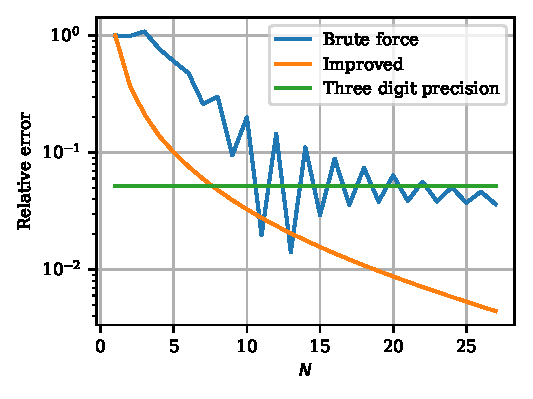
\includegraphics[scale=0.55]{{Figures/exercise_a_b}.pdf}
	\caption{Figure showing the relative error for the brute force gaussian quadrature and the improved gaussian quadrature methods, described in section \ref{subsec:brute_force_gauss} and \ref{subsec:improved_gauss} respectively, as a function of grid resolution $N$. A line is drawn when the relative error is $10^-2$ to illustrate when the integral reaches three digit precision.}
	\label{fig:relerrquad}
\end{figure}
The relative error was also compared for both the brute force Monte Carlo method
and the improved Monte Carlo method described in section
\ref{subsec:brute_force_monte_carlo} and \ref{subsec:improved_monte_carlo}
respectively. This is shown in figure \ref{fig:rellerrcarlo}. For the same
calculations using both Monte Carlo methods, the variance was also plotted. This
is result is illustrated in figure \ref{fig:variancecarlo}. 
\begin{figure}[h]
	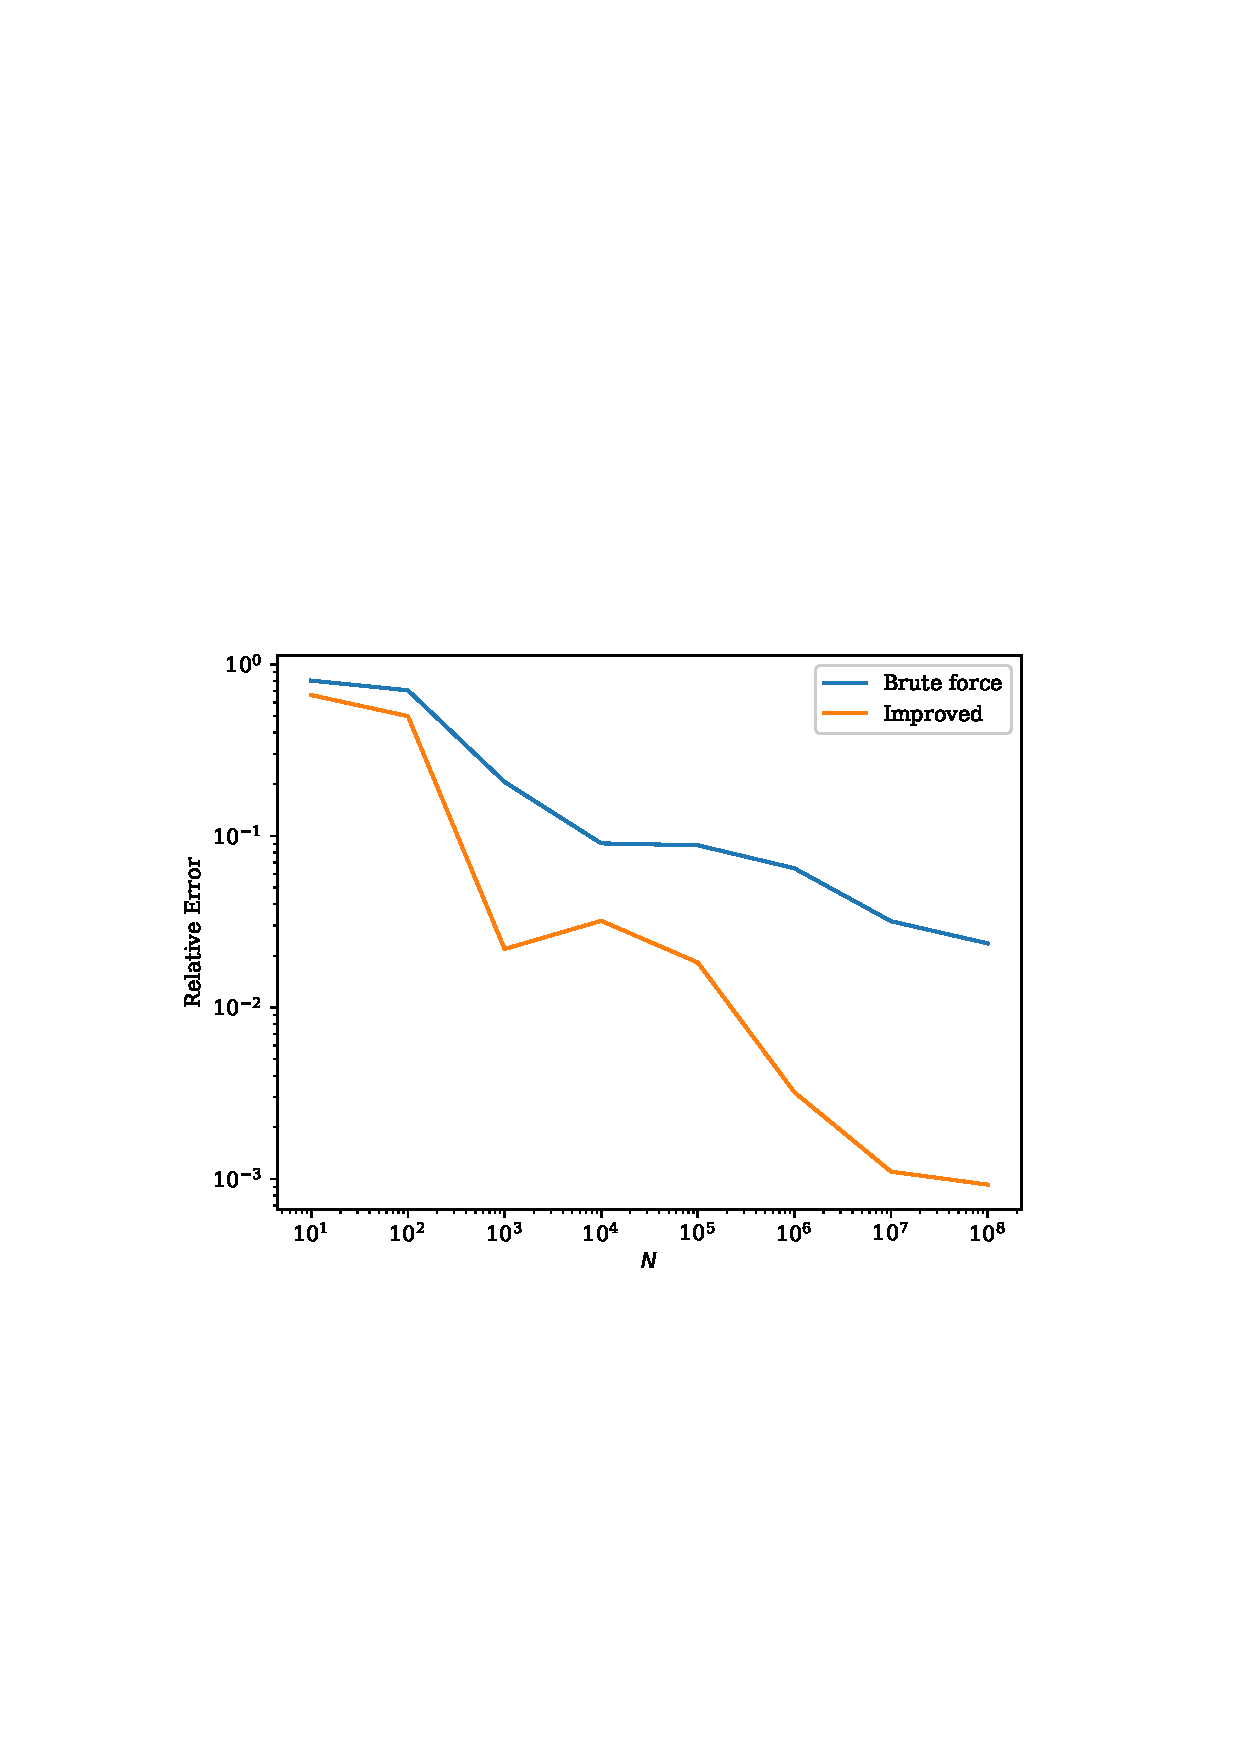
\includegraphics[scale=0.55]{{Figures/error_monte_carlo}.pdf}
	\caption{Figure showing the relative error for the brute force and the improved Monte Carlo methods, described in section \ref{subsec:brute_force_monte_carlo} and \ref{subsec:improved_monte_carlo} respectively, as a function of the sample size $N$.}
	\label{fig:rellerrcarlo}
\end{figure}

\begin{figure}[h]
	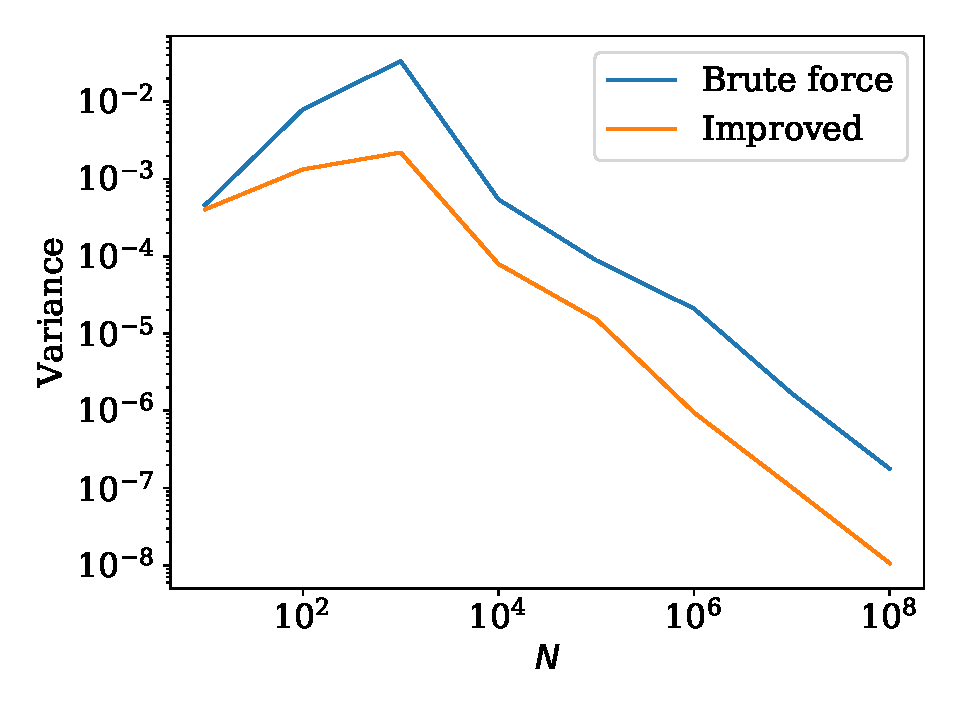
\includegraphics[scale=0.55]{{Figures/variance_monte_carlo}.pdf}
	\caption{Figure showing the variance for the brute force and the improved Monte Carlo methods as described in section \ref{subsec:brute_force_monte_carlo} and \ref{subsec:improved_monte_carlo} respectively as a function of the sample size $N$.}
	\label{fig:variancecarlo}
\end{figure}
The CPU time for both the brute force and the improved Monte Carlo methods was
calculated using no parallelization and parallelization with two threads. This
is shown in figure \ref{fig:CPUcarlo}. The three different compiler flags -O1,
-O2 and -O3 was also compared to study their impact on the CPU time, which is
shown in figure \ref{fig:CPUcarloflag}. This result was produced using
parallelization with four threads.
\begin{figure}[h]
	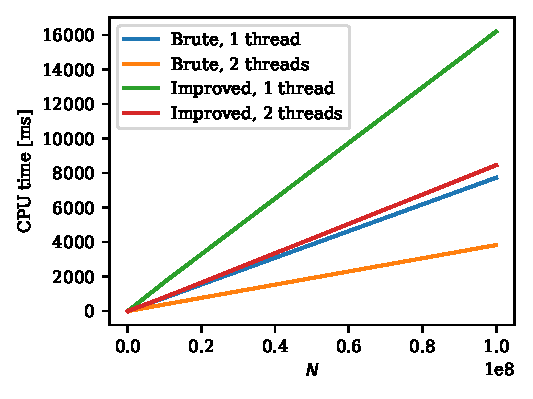
\includegraphics[scale=0.55]{{Figures/cpu_time_monte_carlo}.pdf}
	\caption{Figure showing the CPU time the brute force and the improved Monte Carlo methods, described in section \ref{subsec:brute_force_monte_carlo} and \ref{subsec:improved_monte_carlo} respectively, as a function of the sample size $N$. For both methods the CPU time was compared both unparallelized and parallelized with two threads.}
	\label{fig:CPUcarlo}
\end{figure}

\begin{figure}[h]
	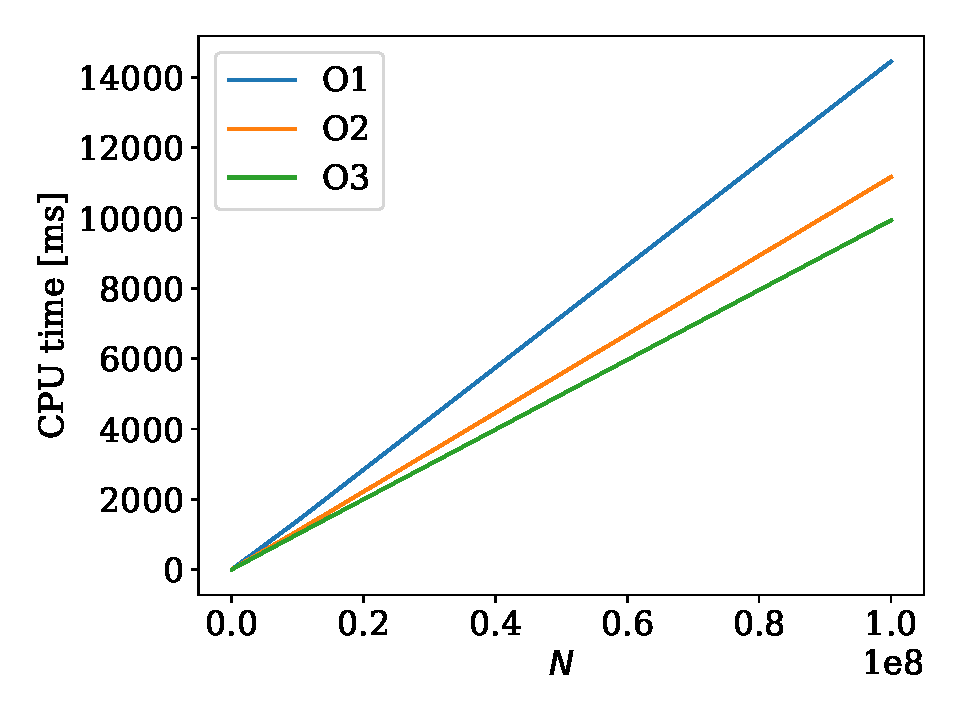
\includegraphics[scale=0.55]{{Figures/cpu_time_compilerflag}.pdf}
	\caption{Figure showing showing the CPU time for the improved Monte Carlo method, described in section \ref{subsec:improved_monte_carlo}, as a function of the sample size $N$ using the different compiler flags -O1, -O2 and -O3. These results were produced using parallelization with four threads.}
	\label{fig:CPUcarloflag}
\end{figure}
\section{Discussion} \label{sec:discussion}
\section{Conclusion} \label{sec:conclusion}

\nocite{jensen:2019}
\bibliographystyle{aasjournal}
\bibliography{ref}

\end{document}

